\openingarticle
\def\ppages{\pagerange{verdu:firstpage}{verdu:lastpage}}
\def\shorttitle{Unearthing the Roads of Roman Hispania}
\def\maintitle{Unearthing the Roads of Roman Hispania: Evolution of Theories, Methodologies and Value Enhancement Techniques}
\def\shortauthor{Antonio Sánchez Verdú}
\def\authormail{antonio\char`_asv19@hotmail.com}
\def\affiliation{University of Alicante: \\ Department of Prehistory, Ancient History and Archaeology}
\def\thanknote{\footnote{Antonio Sánchez Verdú holds a BA in History (2013) and a Master's degree in Professional Archaeology and Heritage Management (2014) from the University of Alicante, Spain. Currently, he is finishing a fellowship contract in the numismatics department of the Archaeological Museum of Alicante (MARQ), and he is also starting his doctorate at the department of Prehistory, Ancient History and Archaeology of the University of Alicante. }}
%--------------------------------------------------------------
\mychapter{\maintitle}
\begin{center}
	{\Large\scshape\shortauthor \thanknote}\\[1em]
	\email \\
	\affiliation
\end{center}
\vspace{3em}
\midarticle
%--------------------------------------------------------------
\label{verdu:firstpage}

	%----------------------------------------------------------------------------------------
	\begin{myabstract}
 Since\marginnote{Abstract\\(in Spanish see below)} the 1980s, the interest in bringing archaeology closer to the public has resulted in attempts to integrate different Roman roads within museums and touristic and cultural itineraries, with varying levels of coherence, historical accuracy and social reception. Despite the increasing proliferation of these projects, aimed to identify, recover and preserve these roads, their methodology was far from uniform until recently. In this paper, I briefly outline the past and current context of the study conditions of the \textit{viae}, due to the shortage of general studies dedicated to the processes of excavation and research of these archaeological remains in Spain. I also try to explain the different value enhancement processes of \textit{viae} for improving public understanding and appreciation of their historical relevance and socio-cultural significance.
	 
\keywords[Keywords]{\textit{Viae}, Roman road, Archaeology, Historiography, Connectivity, Infrastructure, Heritage, Value enhancement, Musealisation.}

	\end{myabstract}
	
%----------------------------------------------------------------------------------------
	%	KEYWORDS
%----------------------------------------------------------------------------------------

%\section{Introduction: Development of the Roman road system in Hispania}
	
	\lettrine[nindent=0em,lines=3]{T}{he} construction\marginnote{Development of the Roman road system in Hispania} of Roman roads in Hispania began with the arrival of the first Roman troops in the late \nth{3} century \BC, and developed, on one hand, by re-using existing roads \parencite[26]{Sillières_2003} and, on the other hand, by creating new routes, in paths previously inaccessible, thanks to Roman technical advances.
	
	During the \nth{2} and \nth{1} centuries\BC the \textit{viae} were adapted and expanded in relation to the war activities developed in Hispania, according to classical authors; however, far from this simplistic view, we should mention other factors such as the improvement of the governance in new conquered territories and access to mining sites: the need for resources to supply the continuous military campaigns promoted the construction of roads towards the most important mining regions (El Bierzo, León, where the famous mines of Las Médulas are located; Tras-o-Montes, north of Portugal, and present-day Galicia, among other gold-rich areas. Also relevant were the silver mines of \textit{Carthago Nova}, currently Cartagena, in the Murcia Region. The Iberian Peninsula was a territory known for its mineral wealth, as referred authors like Strabo, Pliny or Pomponius Mela \parencite[40--49]{Blázquez_1968}, and this did not escape to the Roman greed; since the Second Punic War, private lessees and, after the second century \BC, corporations (\textit{publicani}) systematically exploit Hispanic mineral resources. After the definitive establishment of Roman administration, \textit{viae} were used for political management and tax collection, which contributed to the process of acculturation labelled ‘Romanisation’. Besides, and despite the primacy of maritime trade in commodity exchange, interurban roads played an important role in the transport of products to inner regions.
	
	\textit{Viae} were conceived as \textit{res publicae in usu publico}, that is to say, public, inalienable and costless infrastructure \parencite[63]{Ponte_2007}. We must distinguish three types of roads, according to their characteristics: \textit{viae terrenae}, paved with tamped grit; \textit{silice stratae}, flagstoned roads, and \textit{glarea stratae}, whose surface layer was composed of gravel. Moreover, according to its administrative features, we must differentiate among \textit{viae publicae}, roads financed and maintained by the state; \textit{viae militares}, funded by the military treasury and built at specific times, and \textit{actus} and \textit{viae privatae}, lower roads that completed the road network at regional and local level.
	
	Since the ‘Crisis of the Third Century’, the road maintenance became a secondary priority in the Roman administration, until the fifth century, when most roads were abandoned. After the decline of the Western Roman Empire, probably some roads and bridges continued being used, due to its excellent quality; however, unnecessary items, such as roads built towards decadent cities, were abandoned. As a result, some roads now rest fossilized under successive reforms in the road network, especially during the eighteenth century, when most of the ‘Cañadas Reales’ (passages for migrating livestock) were built \parencite[14]{Moreno_2010}, and other roads disappeared as communication routes, remaining as agricultural roads or even as boundaries between properties \parencite[11]{Moreno_2010}.
	
%	\section{Origin of the Roman roads’ historiography in Spain}
	
	Since\marginnote{Origin of the Roman roads’ historiography in Spain} the sixteenth century, following a renewed interest in classical culture, some studies stressed the relevance of Roman antiquities. The first meaningful example is the work of Ambrosio de Morales \textit{Las antigüedades de las ciudades de España que van nombradas en la Coronica}, published in 1577 \parencite[13]{Abascal_2012}, which made a brief description of the Antonine Itinerary, identifying it as a ‘booklet’ used to locate roads \parencite[20--22]{Morales_1792}. Although misleading when describing \textit{viae} as exclusively military and administrative roads, it was one of the first historiographical examples of localising Roman roads using ancient sources critically, a custom not very widespread in the sixteenth century \parencite[15]{Abascal_2012}. Another of these early works is the \textit{Itinerarium Antonini Augusti et Burdigalense}, by Jerónimo Zurita, in 1600. This author not only enhanced our understanding of an important source for the study of Iberian roads, he also developed a cursory investigation of some roads quoted by this \textit{itinerarium}. However, despite the great contribution of Zurita to the study of Roman roads, during the seventeenth century it did not change the research approaches and the theoretical landscape of the field.
	
	The first in-depth study of Roman roads was the work of Nicolas Bergier. In the \textit{Histoire des Grands Chemins de l’Empire Romain} \parencite{Bergier_1622}, he made a broad study of French Roman roads, combining the study of ancient texts and the analysis of archaeological remains. Bergier was able to realize a systematic and accurate analysis of the structure of the roads: ‘The gravel is always reserved to the surface of the roads; but in order to ensure that their work was lasting [\ldots] they took care of cement, sustain and fortify the gravel below [\ldots]’, but his study was almost unnoticed in Spain until the eighteenth and nineteenth centuries, when authors like Manuel Fernandez de Mesa and Eduardo Saavedra used this text for their researches \parencite[129--130]{Rodriguez_2010}. Indeed, it was Eduardo Saavedra who promoted the archaeological study of Roman roads in Spain with his work \textit{Descripción de la vía romana entre Uxama y Augustobriga} \parencite{Saavedra_1861}, attending to the techniques used in his work, including first hand observation of the paths and comparison of existing data with ancient materials \parencites[7]{Abásolo_1990}[199]{Arias_2002}.
	
	Turning now to the twentieth century, the ‘Junta Superior de Excavaciones y Antigüedades’ played a major role in the study of Roman roads, supporting the work of authors such as Antonio Blázquez and Claudio Sánchez Albornoz (among others, \textit{Diversas longitudes de las millas romanas}, or the joint work textit{Vías romanas del Valle del Duero y Castilla la Nueva}). Another important author was Manuel Gómez-Moreno, who in the early years of twentieth century developed the Monumental and Artistic Catalogues of the provinces of Ávila, Salamanca, Zamora and León.
	
	After the Civil War, independent scientific production declined. Only since the 1960s have authors like Manuel Roldán and Gonzalo Arias recovered the habit of regular work in the study of ancient road; Roldán with his work about resources for the study of \textit{viae} (\textit{Itineraria Hispana}) and its exhaustive study on the \textit{Via} de la Plata (\textit{Iter ab Emerita Asturicam}) and Arias with his \textit{Repertorio de Caminos de la Hispania Romana} and, above all, the impulse of the magazine \textit{El Miliario Extravagante}. From these years, literary and scientific production has grown considerably, fostering interest about Roman roads, which, in turn, led to numerous publications about the \textit{viae} \parencites{Blázquez_2006}{Chevallier_1997}{Moreno_2004}, such as in relation to their location \parencites{Morote_2002}{Roldán_1971}{Sillières_1990}, their structure \parencite{Moreno_2009}, their related elements \parencites{Arasa_1990}{Rodriguez_2004} or their relevance in the organisation of Roman society \parencites{Pisani_1994}{Ponte_2007}.
\myseparator
\marginnote{Identifying the roads}%	
%	\section{Identifying the roads}
	There are several issues that may arise when identifying the Roman roads; the main one is the confusion about the construction characteristics of the \textit{viae} \parencite[11--12]{Moreno_2010}. Researchers \parencites{Chevallier_1997}{Moreno_2004}{Moreno_2009}{Sillières_1990} have defended until recent years the assumption of the divided structure of these roads (\textit{statumen, rudus, nucleus and summa crusta or summa dorsum}), a theory established in the eighteenth century, following a misreading of Nicolas Bergier \parencite[93--93]{Chevallier_1997}. The image of the Roman roads as paved pathways transcended from academic ambits to public understanding during the nineteenth and twentieth centuries. Although in Roman engineering some sections of tracks were paved, they usually belonged to the inner city or nearby, where the surface was paved in order to avoid the discomfort produced by the dust generated by traffic. Moreover, paved sections were built in places where the gradient caused fast erosion of the surface layer, or, simply, places where the necessary raw materials, such as granite, were abundant \parencite[51]{Rodriguez_2004}.
	
	For the location and identification of the Roman roads there are several useful techniques:
	
%	\subsection{Remote Sensing}
	
	The\marginnote{Remote Sensing} first tool is remote sensing, category encompassing various traditional and modern techniques, such as aerial imagery (see Fig. \ref{fig:verdu_Fig1}). GIS techniques have decisively contributed to both the identification of possible \textit{viae} layouts, and the creation of map databases to provide additional and comparative information about the road system.
	
%	\subsection{Cartography}
	
	Historical\marginnote{Cartography} cartography has also played a major role in associating physical features and place names in order to locate road sections; it is advisable to be wary of the 1920's and 1930's maps \parencite[12]{Moreno_2010}, although some military maps from this period were made on limited areas and with high accuracy. Map information can also be useful for identifying place names related to road items, despite the fact that sometimes their relationship with the Roman world is based on misunderstandings during medieval times.
	
%	\subsection{Prospection}
	
	Another\marginnote{Prospection} essential technique for the identification of Roman roads is prospection, which could be executed through surface analysis or aerial survey. Because of the length and the physical characteristics of our element of study, the best options when we want to recognize them are aerial survey and satellite imaging, techniques which allow us the identification of optimal locations for roads \parencite[412]{Sillières_1990}, and the evidences of the \textit{viae} by the identification of vegetation changes \parencite[416]{Sillières_1990}. On the other hand, surface survey allows recognition of the visible remains of the tracks, but also, of their destroyed remains, which leave archaeological evidence in the form of infilled side ditches, scattering of building materials or remains from the gathering and transport of construction materials \parencite[31]{Moreno_2009}.
	
%	\subsection{Analysis of the formal conditions of the road}
	
	The\marginnote{Analysis of the formal conditions of the road} most useful technique for identifying \textit{viae} is through structural analysis, by archaeological excavation or field survey. Roman engineers used specific materials, obtained and placed in a planned way along a concrete geographical route and according to some defining technical characteristics of Roman engineering. I summarize below some of those items that allow a correct identification of Roman \textit{viae}:
	
	%FIGURE 1 HERE
	\begin{figure}[!htb]
		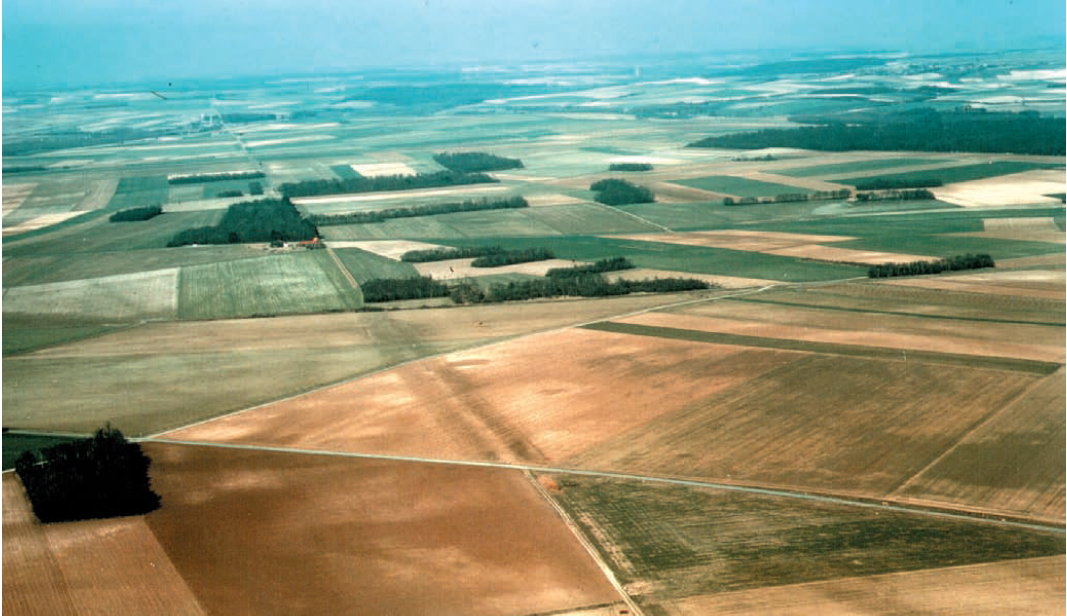
\includegraphics[width=\linewidth]{figures/verdu_Fig1}
		\caption{Aerial photography where evidence of a very long straight section of the Via from Amiens to Senlis, in Oise Valley, France, can be appreciated. Source: \textcite[147]{Moreno_2004}. Photograph: R. Agache (used with copyright-holder’s permission).}
		\label{fig:verdu_Fig1}
	\end{figure}
	
	\begin{enumerate}
		\item The roads were built along a longitudinal trail (i.e., avoiding tortuous paths) (Fig. \ref{fig:verdu_Fig1}). This can serve us as a general indicator of its chronology when we have no physical evidence of the track structure \parencites[362--363]{Arasa_2008}[415]{Sillières_1990}, although I argue that a road should never be identified by only following this approach \parencite[14]{Abásolo_1990}, and other indicators must be sought.
		\item In mountainous paths, roads maintained slopes lower than \SI{8}{\percent}, making huge constructive efforts into planning the route, for example, by designing the ascension in strategic points in order to maintain a prolonged climb and a regular slope \parencites[15]{Abásolo_1990}[21--22]{Moreno_2009}.
		\item Interurban roads \parencite[417]{Sillières_1990} are composed of bottom layers of large stones regularized by a layer of fine materials, whereas in the upper layers stratums of fine-grained ballast which function as surface layer (Fig. \ref{fig:verdu_Fig2}). This ballast must be tough in order to endure traffic, and quite rounded to avoid damages to the animals’ hooves \parencite[28]{Moreno_2009}. Alternatively, the whole structure can be constructed by superimposing and compacting fine layers, from \num{10} to \SI{15}{\centi\meter} thick \parencite[23]{Moreno_2009}, until obtaining adequate quality standards for transit. 
	\end{enumerate}
	
	%FIGURE 2 HERE
	\begin{figure}[!htb]
		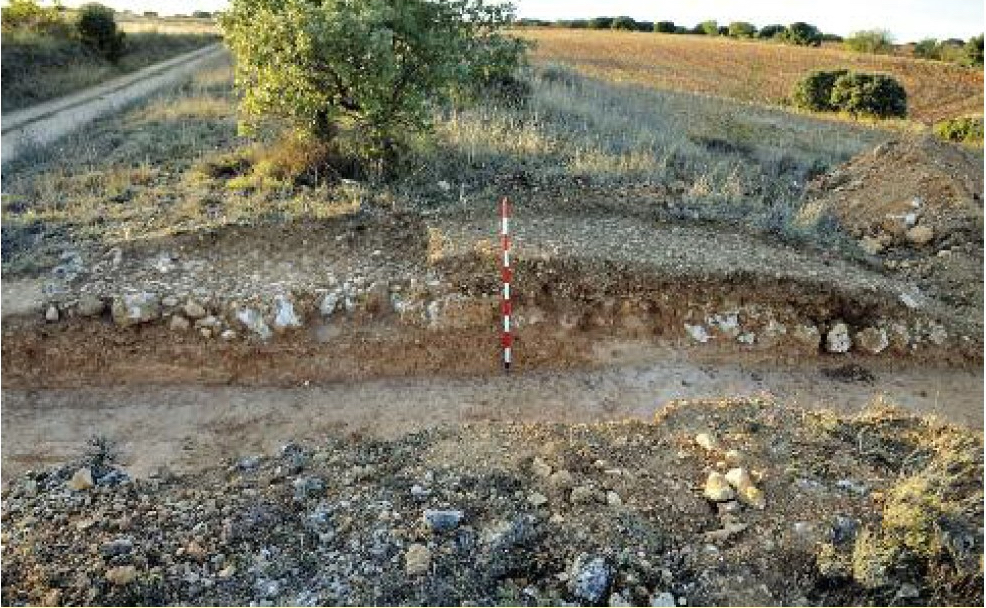
\includegraphics[width=\linewidth]{figures/verdu_Fig2}
		\caption{Photography of the Via from Clunia to Segisamo (Castille and León), where the foundation of large limestone rocks and a surface layer of natural ballast over it can be appreciated. Source: \textcite[24]{Moreno_2004} (used with copyright-holder’s permission).}
		\label{fig:verdu_Fig2}
	\end{figure}	
%	\subsection{Ancient sources}
Very \marginnote{Ancient sources} briefly, I present the three most important sources for Hispania, described in more detail by \textcite{Roldán_1975}. Other ancient sources refer to the construction of roads butdo not contribute to locate them, like the Book~VII of Vitruvius, references in Pliny’s Natural History or poet Statius’ \textit{Silvae}. Moreover, other sources like the \textit{Tabula Peutingeriana}, the \textit{Itinerarium maritimum} or epigraphic documents like the \textit{Tegula} of Valencia or the clay tablets of Astorga, either make a partial list of the roads, or they lack the geographical precision needed to make a reliable identification \parencites[3]{Arias_1987}[102--175]{Roldán_1975}.
	
	\begin{enumerate}
		\item Vicarello Goblets: They are four small silver glasses discovered in 1852, after the demolition of the thermal baths of Vicarello, formerly known as \textit{Aquae Apollinares Novae}. On their surface, the 104 stations on the route between \textit{Gades} (Cádiz) and Rome are engraved, totalling 1840 miles \parencite[104]{Benítez_2012}.
		\item \textit{Itinerarium Provinciarum Antonini Augusti}: Also known as Antonine Itinerary, it is a compilation of notes of 372 itineraries. Of these routes, 34 are within the Iberian Peninsula. It was probably made in the third century, and it was based on travels and descriptions.  \parencites[83--116]{Arias_1987}[38--101]{Roldán_1975}.
		\item Ravenna’s Cosmography: Dating from the seventh century, it was possibly based on the \textit{Tabula Peutingeriana} and other contemporary maps, especially from the third century \parencite[112--113]{Roldán_1975}. In some chapters of the books IV and V it refers to the \textit{viae} of Hispania. Its main issue is that it does not describe ways, but lists of cities grouped by proximity.
	\end{enumerate}	
%	\subsection{Epigraphic evidence}	
	The\marginnote{Epigraphic evidence} study of epigraphic elements, mainly milestones, is especially useful in areas where they are frequently preserved, as northwest Spain \parencite[30]{Rodriguez_2004}, while on roads where their presence is poorer, as in the eastern part of the peninsula, other sources of evidence are required. The information given by milestones located on the same road can be synchronous, i.e. milestones placed at the time of construction, or diachronic, because repairing roads could lead to the erection of new milestones \parencite[159--160]{Moreno_2004}. 
	
	Nonetheless, the epigraphic evidence is not restricted to milestones; there are lower markers which could indicate half miles (instead of \textit{millia passuum} indicated by milestones), fixed directional signs at intersections, near the cities or at the stations and \textit{mansiones}, and even elongated sticks to demarcate the layout of the road in case of snow \parencite[161--164]{Moreno_2004}. Furthermore, altars dedicated to the \textit{Lares Viales}, relatively frequent on roadways, honorary inscriptions or funerary monuments can also provide further evidence for the presence of a Roman road \parencites[759--766]{Rodriguez_2004}[73--75]{Chevallier_1997}.
	
	Even with all these techniques and lines of evidence, there are still two main issues with the road investigation process. The first problem is related to the interpretation of the itineraries, generated by wrong explanations made during the nineteenth century, when some scholars suggested possible itineraries for different roads \parencite[47]{Beltrán_1990} without much supporting literary or epigraphic evidence. The second problem is the confusion between Roman roads and other posterior infrastructure, such as the aforementioned ‘Cañadas Reales’. In this particular case, as previously mentioned the common mistake is to consider that all Roman roads were flagstoned or cobbled superficially, and because of this, some researchers and members of the public may still misidentify them.
	
%	\section{Excavation process}
	
	The\marginnote{Excavation process} excavation of roads does not currently follow the standard procedures of archaeological excavation and documentation, because the classical stratigraphic method is not particularly useful when studying contemporary constructive levels, not even in cases where two roads overlap \parencite[36]{Moreno_2009}.
	
	When excavating a Roman road, its structural design should be considered first (ideally during the identification process), differentiating artificial layers from the natural substrate; only after this action can the right excavation process be planned, in order to obtain the highest amount of information from the different building phases \parencite[49]{Palomino_2010}. This planning process is more appropriate than the classical stratigraphic method because the succession of layers that compose the road is a functional and artificial stratification, so the usual archaeological excavation would only cause the destruction of the \textit{viae} layer by layer, without obtaining information, and, in many cases, even without detecting the different construction phases of the road correctly.
	
	To reaffirm the difficulty of applying the stratigraphic method to the excavation of \textit{viae}, I note that it would be practically impossible to find any archaeological element over the construction layers because it would be unlikely that a worthless object had survived centuries of transit across the road, or, conversely, that no one had picked up a valuable object dropped on the road. One exception are the \textit{clavi caligarii}, metal nails on the soles of the \textit{caligae} \parencite{Rodriguez_2012}. These nails allow us to date with relative precision the Roman roads or, at least, differentiate them from those in which the material findings indicate later periods. Nevertheless, the hypothetical discovery of archaeological remains in the surface layers of the roads is generally of limited use, because taking this finding as a benchmark within the broad chronological range of road use can lead to a dating error or to a partial analysis. On the other hand, the few materials that could be recovered within the structure would be mixed with building materials, of unknown geographical and temporal origin \parencite[36]{Moreno_2009}. Although they could provide a \textit{post quem} date, this would not provide a precise chronology for the construction and use of the road.
	
	Therefore, after ruling out the stratigraphic method, we identify two advisable techniques for the correct excavation and study of the roads: the first one involves obtaining transverse or longitudinal sections (Fig. \ref{fig:verdu_Fig3}), either through cleaning or digging, allowing the identification of the construction sequence in an easy and visual way. The second technique is the excavation of the layers by stepped sections, (Fig. \ref{fig:verdu_Fig4}) to differentiate them while, at the same time, gathering information about the construction process \parencite[49]{Palomino_2010}, such as tread marks of vehicles used during the construction. In this second process, the nature of the building materials must be taken into account, because this excavation will be considerably easier in the surface layers and other fine layers, than in the rocky foundations \parencite[35]{Moreno_2009}.
	
	The correct excavation of these roads provides information about its constructive methodology and its structure, and also confirms or refutes its ascription to Roman period \parencites[33]{Moreno_2009}[72]{Palomino_2010}. 
	
		%FIGURE 3 HERE
		\begin{figure}[!htb]
			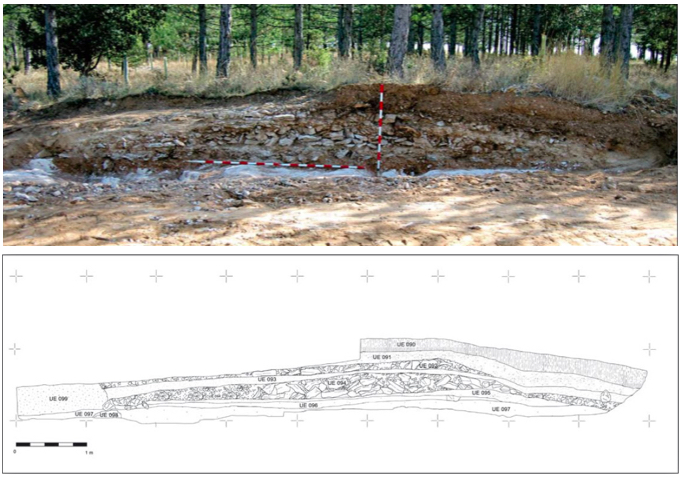
\includegraphics[width=.9\linewidth]{figures/verdu_Fig3}
			\centering
			\caption{Photography and drawing of the archaeological work at the Via from Clunia to Segisamo through a transverse cleaning of the structure. Source: \textcite[56]{Palomino_2010}. Photograph: Aratikos Arqueólogos, S.L. (used with copyright-holder’s permission).}
			\label{fig:verdu_Fig3}
		\end{figure}
		
		%FIGURE 4 HERE
		\begin{figure}[!htb]
			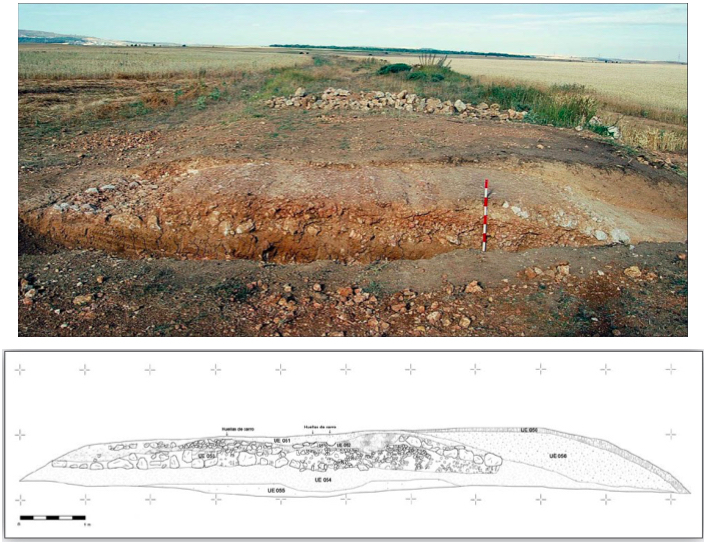
\includegraphics[width=.95\linewidth]{figures/verdu_Fig4}
			\centering
			\caption{Photography and drawing of the archaeological work at the Via from Italia to Hispania through stepped sections. Source: \textcite[64]{Palomino_2010}. Photograph: \textit{Aratikos Arqueólogos}, S.L. (used with copyright-holder’s permission).}
			\label{fig:verdu_Fig4}
		\end{figure}	
%	\section{Restoration and musealisation projects}	
Archaeological\marginnote{Restoration and musealisation projects} excavation is not the last research phase for understanding and presenting Roman roads. To ensure that the acquired archaeological knowledge is useful, the information obtained should be presented to the public, thus creating further interest about the meaning of heritage, its importance and the need to take care of it; an appropriate procedure is through the musealisation or exhibition of the remains. However, the presentation of their remains is not commonplace yet, and the process of restoring Roman roads is not homogeneous. There are several criteria to take into consideration, in relation to the different types of \textit{viae}. In order to illustrate them, I present three case studies, corresponding to three types of roads, with the aim of showing the particularities of each one. 

%\subsection{Main roads: ‘Vías Atlánticas’ Project (Galicia)}

‘Vías Atlánticas’ \marginnote{Main roads: ‘Vías Atlánticas’ Project (Galicia)} is a program designed to study, preserve and raise awareness of the \textit{viae} XIX and XX of the Antonine Itinerary, which connected the cities of \textit{Bracara Augusta} (Braga, Portugal) and \textit{Asturica Augusta} (Astorga, Spain), through \textit{Lucus Augusti} (Lugo, Spain). It also involves the creation of a joint touristic heritage site, integrating these regions. The project propose a unitary track that links these two roads, idea which, despite some criticism, is not implausible if we consider the connected structure of Roman itinera.
The project developed in four phases: 
\begin{enumerate}
	\item Planning: definition of the project to encourage cooperation between all the agencies involved, and to establish responsibilities, activities to be carried out, and planned schedule.
	\item Archaeological interventions: demarcation of the roads’ layout, inventory of archaeological and artistic elements, excavations at selected locations and additional scientific research. A source of controversy in the study of these routes is the diversity of sources: Antonine Itinerary, Ravenna Cosmography, clay tablets of Astorga \parencites[149]{Mendez_1996}[22--30]{Rodriguez_2004}, in addition to the information obtained from archaeological elements, such as \textit{mansiones}, milestones and \textit{Lares Viales} altars \parencite{Rodriguez_2004}. This fact, combined with the degradation of the \textit{viae}, complicated the study process.
	\item Marketing: Creation of a website (\url{http://viasatlanticas.depo.es/}), development of suitable materials for tourist interpretation, edition of teaching guides and organization of exhibitions, workshops and scientific publications (Fig. \ref{fig:verdu_Fig5}).
	\item Conservation: cleaning and maintenance tasks, always under specialised counselling in order to stimulate the preservation of the paths. 
\end{enumerate}

	%FIGURE 5 HERE
	\begin{figure}[!htb]
		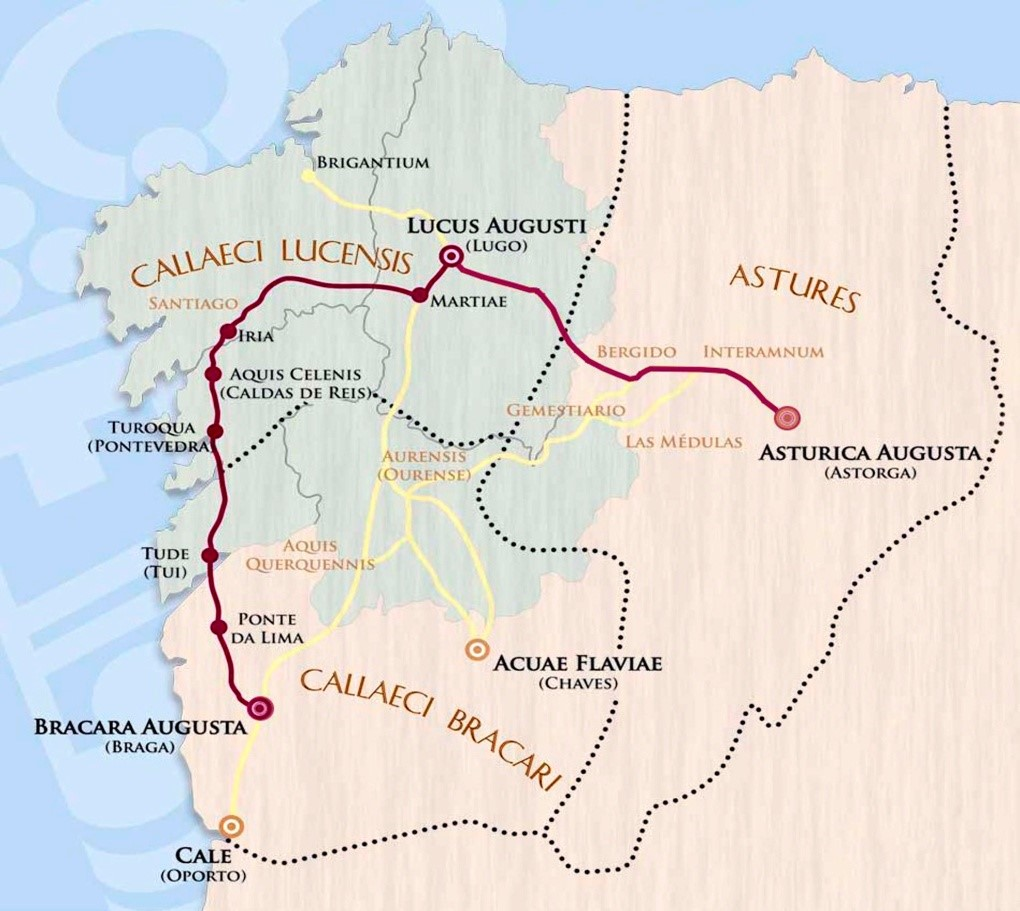
\includegraphics[width=\linewidth]{figures/verdu_Fig5}
		\caption{Official informative \url{http://viasatlanticas.depo.es/promocion/MAPA\%20VIA\%20XIX\%20EPOCA\%20ROMANA.jpg} of the ‘Vías Atlánticas’ Project.}
		\label{fig:verdu_Fig5}
	\end{figure}	
%\subsection{Urban roads: ‘Vía del Pórtico’ (Sagunto, Valencian Community)}
\noindent This\marginnote{Urban roads: ‘Vía del Pórtico’ (Sagunto, Valencian Community)} archaeological site has been integrated in a musealisation project that includes architectural elements from the second century to medieval times. Particularly relevant is a segment of urban road, remarkable for the preserved evidence of the portico built on either side of it, and for the extraordinary level of preservation of the paving stones. During the second century, this road was the \textit{kardo maximus} of \textit{Sagvntum}, that is to say, the main street of Sagunto; its width was between \SI{4.10}{\meter} and \SI{5.40}{\meter}  \parencite[15--17]{Melchor_2005a}. Adding the arcaded sidewalk, it would have reached about \SI{8}{\meter} in width (Fig. \ref{fig:verdu_Fig6}). Maybe this \textit{strata}, or urban paved street, was connected with the \textit{Via Augusta} outside of the city; it is even possible that the ‘Vía del Pórtico’ was the extension of the \textit{Via Augusta} inside \textit{Sagvntum} \parencite[15]{Melchor_2005a}, although this assertion cannot be determined with certainty. The earliest archaeological activities were executed in 1992, when the construction of a building was planned on an abandoned plot that had previously been occupied by a football pitch. The emergence of structures during development fostered the beginning of an archaeological excavation that lasted until 1994.

	%FIGURE 6 HERE
	\begin{figure}[!htb]
		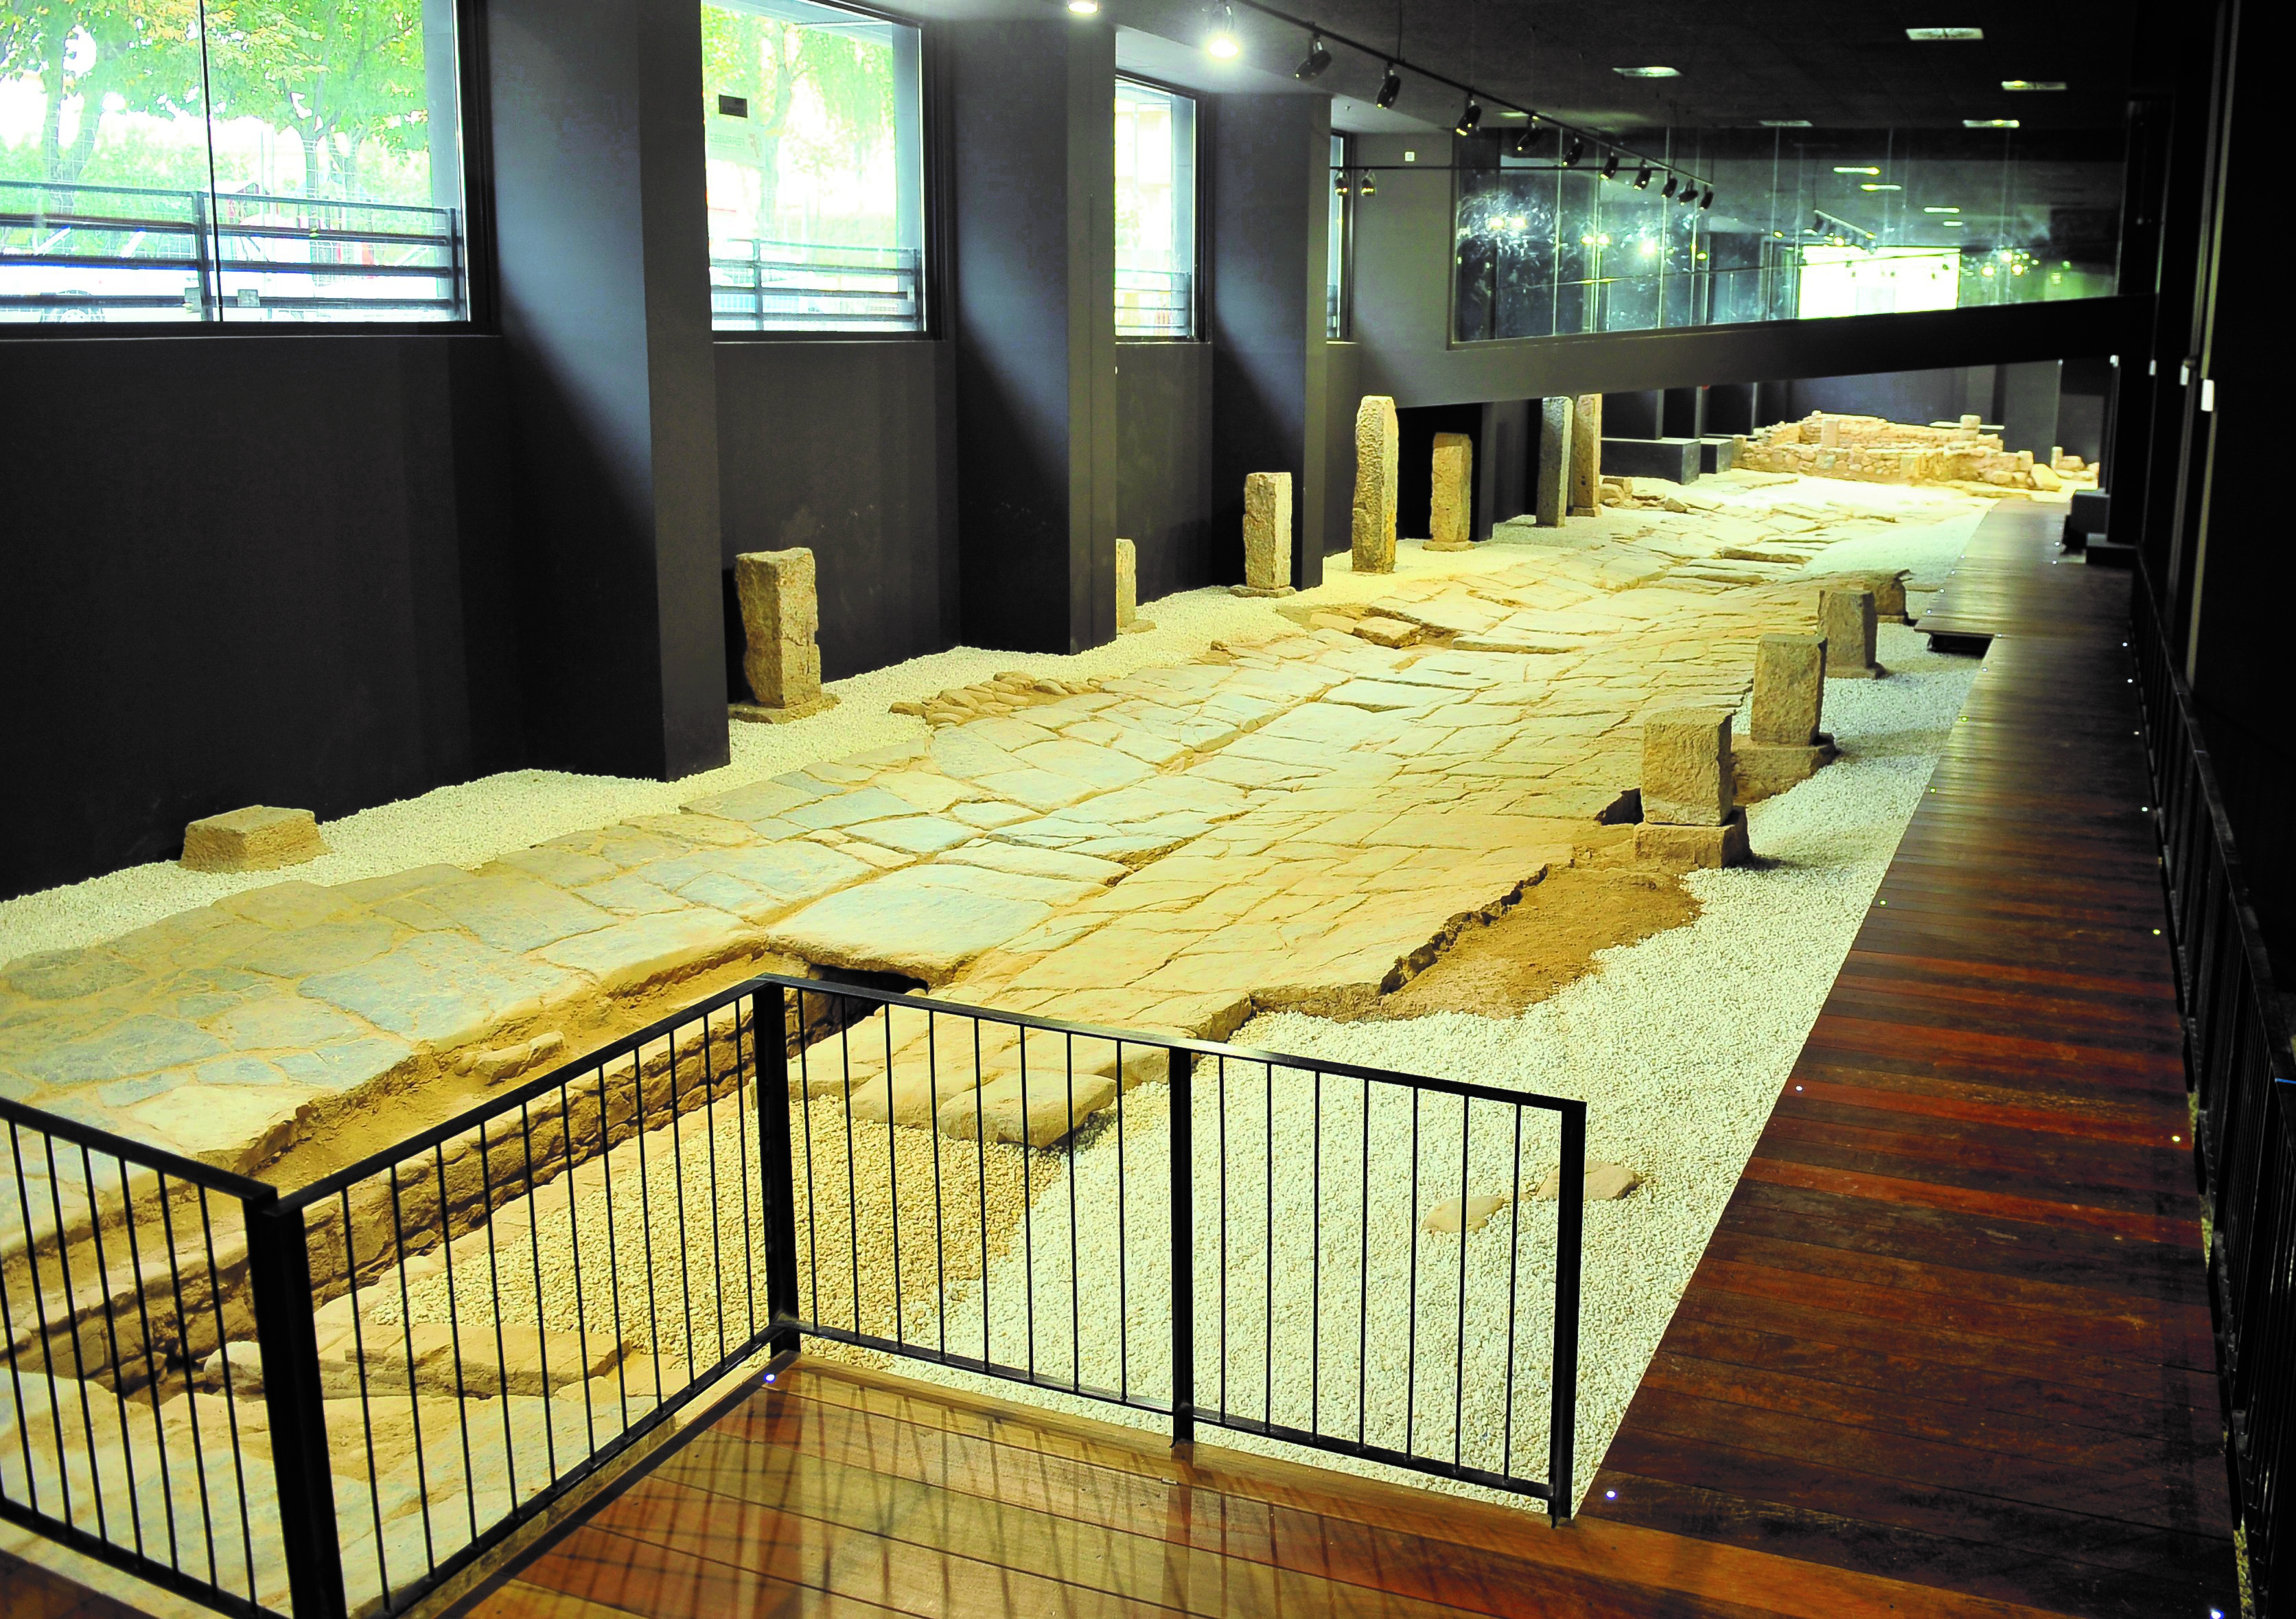
\includegraphics[width=.9\linewidth]{figures/verdu_Fig6}
		\centering
		\caption{Image of the road inside the ‘Vía del Pórtico’ Museum. Photograph: Higueras (courtesy of Sangunto City Hall, used with copyright-holder’s permission).}
		\label{fig:verdu_Fig6}
	\end{figure}
	
By 1994, three roman rooms and several other structures damaged by medieval buildings were documented and excavated, as well a little alley which, in its western end, joined with the main road.

Between 2002 and 2004, further building development led to the expansion of the excavation area to the north, where the most outstanding findings were found, including the paved road that focuses our interest. The archaeological project was carried out through open-area excavation, where the grey limestone flagstones of the \textit{via} were unearthed. This process was performed manually, using machinery only for the clean-up and the removal of surface layers \parencite[323]{Melchor_2005b}. 

The process of value enhancement of the ‘Vía del Pórtico’ started in 2006. It consisted, first, on the excavation and removal of some medieval structures, prioritising Roman infrastructure \parencite[326]{Melchor_2005b}; after which the actual valorisation began, lasting until 2013, with the provision of suitable facilities for a tour around the archaeological remains, and the installation of the necessary museological elements.

%\subsection{Mountain paths: Roman road of ‘La Carisa’ (Asturias)}

The\marginnote{Mountain paths: Roman road of ‘La Carisa’ (Asturias)} third project is the Roman road of ‘La Carisa’, route that crosses the Cantabrian Range between Asturias and León. It is a \textit{via} of about \SI{4}{\meter} wide, with large straight sections built, in some cases, on embankments and, in other cases, carved on the rock \parencites[383]{Camino_2010}[181]{González_2011}. 

This path, unlike some other mountain trails, can be confidently ascribed to Roman times, due to the presence of archaeological evidence in the form of epigraphic texts (milestones and altars) and bridges, such as Olloniego Bridge \parencite[179--180]{González_2011}, whose dating is essential. This hypothesis is confirmed by the data obtained from the discovery and excavation of a military camp on Mount Curriechos. Its occupation period, around 25\BC, coincides with the road construction process \parencites[376--377]{Camino_2010}[180]{González_2011}.

Furthermore, I would like to mention the archaeological excavations dedicated, exclusively, to interpret the road correctly, test the initial hypotheses and strengthen the theories derived from the data. These excavations unearthed the structure of the road, showing that their constructive disposal corresponds to the formal canons of Roman \textit{viae terrenae}, something like dirt roads \parencite[180]{González_2011}. Documentary sources also corroborate the Roman origin of ‘La Carisa’, whose construction is attributed to the general Publio Carisio, governor of the \textit{Ulterior} province during the Cantabrian Wars, around 25 B.C. \parencite[377]{Camino_2010}. I argue that this road was, indeed, a \textit{via terrena} built in the late first century B.C., that survived as a mountain pass, just like other trails across the Cantabrian Range. The principal difference with other roads is that ‘La Carisa’ was not subsequently changed, and it has retained its original construction components.

Finally, in relation to value enhancement, ‘La Carisa’ is publicised as one of the official trekking routes of Asturias. This public scheme offers historical background and details about the construction of the road, its development in Roman times and its socio-cultural significance, in addition to practical information for hikers.

%\section{Conclusions}

%\subsection{Research}

First,\marginnote{Conclusions -- Research} I argue that it is inappropriate to automatically identify paved roads with Roman \textit{viae}. This association has caused numerous mistakes, sometimes even incorrect identification, in the archaeological heritage of roads and paths. Only some \textit{viae}, with concrete features and located in certain areas, have this peculiarity, and are a minority in relation to the \textit{viae terrenae}.
 
In addition, I have described some of the most important techniques for the identification and location of Roman roads. However, no single technique offers total reliability and these techniques should be combined to achieve more reliable research results. Furthermore, the excavation of a \textit{viae} is not primarily performed using the stratigraphic method of archaeological research. In contrast, stepped sections or transverse and longitudinal sections are more appropriate methodologies for the study of Roman roads.

%\subsection{Valorisation of Roman roads}

About\marginnote{Conclusions -- Valorisation of Roman roads} the enhancement of the perceived public value of \textit{viae}, I consider that the final aim of these projects must be remembered: to offer accurate information about the Roman period, and offer it not only to academic circles through scientific publications, but also to the general public, allowing everyone to learn more about the past. I argue that musealisation projects are useful for achieving this aim. 

I propose some common dimension in the process of value enhancement of Roman roads in Spain. As a preliminary step, a Master Plan should be designed, establishing work teams and activities to be undertaken, involving governments (local, regional and/or national) in the project. In addition, it is paramount to obtain funding for the development. An interesting option would be to seek sponsorships from private companies or explore further possibilities for governmental funding.

About the concrete process of enhancement, the first step is recognising the accurate location of the road. This phase will be easier if the \textit{via} is a main interurban road, because more information about it would be available. Then, the activity should focus on archaeological excavations, in order to expose the structure of the road and confirm its origin.

The preservation of the remains is another fundamental step. With the aim of improving their legal protection, applying for heritage distinction to governmental agencies is an interesting option: the road could be included in the Heritage of Cultural Interest (BIC by its Spanish acronym) register or, at least, in the local records of archaeological sites. In the case of urban roads, usually their finding coincides with construction above the remains, so the protection of the site in the early stages of land-use planning is essential.

Finally, these projects should include a promotion plan. Initiatives such as collaboration with museums, coordination of conferences and exhibitions and on-line promotion are key factors in raising public awareness about the importance and the historical significance of these \textit{viae}.

%\subsection{Positive effects of the value enhancement of heritage}

I \marginnote{Conclusion -- Positive effects of the value enhancement of heritage} highlight the benefits that recovered heritage has for local communities, society, governments and/or the economy. In rural areas, the recovery of former roads allows, for example, the adaptation of formerly unused paths for trekking or cycling, offering added value to Sport Tourism. Furthermore, in mountainous paths, the obtaining of funding for the recovery of \textit{viae} could improve access to the landscape while increasing its protection. Finally, the revalorisation of large routes entails inter-regional collaboration, partnership that, if managed appropriately, can be mutually positive, leading to more joint projects in the future. 

In urban areas, the benefits of preserving historical heritage are already well known. I would like to stress its touristic potential, especially if the main heritage assets of the city are connected and jointly managed, thereby facilitating access to these sites through delineated routes. Moreover, in urban areas, the increase of touristic elements is, in most cases, a positive factor, given that it contributes to fostering the activity of other local businesses, such as hotels, restaurants, shops, airports or taxis, among others. Nevertheless, cultural projects should be adapted to the city’s touristic requirements and capacities.

%\subsection{Perspectives for action}

I \marginnote{Perspectives for action} briefly outline some potential future possibilities for research into Roman roads in Spain:

\begin{enumerate}
	\item Creation of a reliable map of the roads of the Iberian Peninsula, based on the techniques discussed above, in order to prevent their destruction by construction, neglect or vandalism. In order to achieve this objective, ‘natural’ pathways should also be considered as areas of potential archaeological relevance.
	\item Considering that the majority of Roman roads are superimposed over other ancient routes, it would be plausible the application of the same research methodology into other periods, in order to offer a more complete sequence of the development of the road system in the Iberian Peninsula. This idea would be particularly useful in value enhancement schemes, because it would allow the public appreciation of the different phases of use of the \textit{viae}.
	\item As already mentioned, the final aim of research and value enhancement is to inform about the characteristics of the \textit{viae} and their need for protection. This goal is not trivial, because citizens are ultimately the holders of heritage and they are responsible for its preservation. Only by emphasising this fact may a civic consciousness of duty towards public heritage be achieved. The best protection for cultural assets is provided by their rightful owners, all of us.
\end{enumerate}
\myseparator
%\section{Acknowledgements}
First,\marginnote{Acknowledgements} I would like to thank the IJSRA team for the opportunity given, and also the assistance and the warm and kind treatment that I have received. Furthermore, I am very grateful to the several authors who have allowed me show their images and have helped me during my research: \textit{Aratikos Arqueólogos}, the team of the Museum of the \textit{Vía Del Pórtico} and Isaac Moreno.


\begin{myabstract}\foreignlanguage{spanish}{%	 	
	 	Desde\marginnote{Abstract (Spanish)} los años 80, el interés por acercar la arqueología al público ha resultado en diversos intentos de integrar la presencia de calzadas romanas en museos y en rutas turísticas y culturales, con unos niveles de coherencia, fidelidad histórica y recepción social variables. A pesar del considerable incremento en el número de este tipo de proyectos con el objetivo de identificar, recuperar y conservar las calzadas, las metodologías empleadas han sido dispares hasta hace relativamente poco tiempo. En el presente artículo introduzco brevemente el estado de la cuestión de las condiciones de estudio de las calzadas, ya que considero que existe una cierta limitación en estudios generales que aborden la excavación e investigación de estos restos arqueológicos en España. También trataré de explicar los distintos procesos de revalorización patrimonial de las calzadas romanas, los cuales tienen por objetivo mejorar la percepción pública de la relevancia histórica y social que representan las calzadas romanas.}
	 	
	 	\keywords[Puntos]{Calzadas Romanas, Arqueología, Historiografía, Conectividad, Infraestructura, Patrimonio, Revalorización, Musealización.}

\end{myabstract}
	%----------------------------------------------------------------------------------------
	%	REFERENCE LIST
	%----------------------------------------------------------------------------------------

\printbibliography[heading=subbibnumbered] 
\label{verdu:lastpage}
\closingarticle